\documentclass[review,12pt]{elsarticle_summary_report}
\usepackage[top=1.0in, bottom=1.0in, left=1in, right=1in]{geometry}


%%%%%%%%%%%%%%%%%%%%
\usepackage{amsfonts}
\usepackage{amssymb}
% \usepackage{MnSymbol}
\usepackage{graphicx}
\usepackage{courier}
\usepackage{psfrag}
\usepackage{amsmath}
\usepackage[usenames]{color}
\usepackage{leftidx}
\usepackage[small]{subfigure}
\usepackage{stmaryrd}
\usepackage{amsthm}
\usepackage{multirow}
\usepackage[table]{xcolor}
% \usepackage{natbib}
\usepackage{nomencl}
\usepackage{setspace}
\usepackage{dcolumn}% Align table columns on decimal point
\usepackage{bm}% bold math
\usepackage{pdflscape}
\usepackage{soul}
\usepackage{parskip}
\usepackage{algorithm}
\usepackage[noend]{algpseudocode}
% \usepackage{showkeys}
%%%%%%%%%%%%%%%%%%%%

\usepackage{hyperref}
\hypersetup{
    colorlinks=true,
    linkcolor=blue,
    filecolor=magenta,      
    urlcolor=cyan,
}

% \usepackage[active,tightpage]{preview}
% \PreviewSnarfEnvironment[{[]}]{figure}

\makenomenclature

\graphicspath{ {./Figures/cav_17_results/}
               {./Figures/pillbox_coarse_uniform_results/}   
               {./Figures/geom_inquires_impl/}   
             }

%\renewenvironment{equation}[0]{equation}{equation}

%%%%%%%%%%%%%%%%%%%% Additional Commands
\newcommand{\bs}[1]{\boldsymbol{#1}} 
\newcommand{\pr}[1]{\left( #1 \right)} 
\newcommand{\br}[1]{\left[ #1 \right]} 
\newcommand{\cbr}[1]{\left\lbrace #1 \right\rbrace} 
\newcommand{\abs}[1]{\left | #1 \right |} 
\newcommand{\mref}[2]{(#1)$_{\text{#2}}$} 
%%%%%%%%%%%%%%%%%%%%
%\numberwithin{equation}{section}  	%%Equation Numbering
%%%%%%%%%%%%%%%%%%%%
\begin{document}

\title{PROGRESS REPORT}% Force line breaks with \\
%\thanks{}%

\author[]{Morteza H. Siboni \\
Gerrett Diamond \\
Cameron W. Smith}
%\ead{email address}

%\author[inst1]{Corresponding Author \corref{cor1}}
%\cortext[cor1]{Corresponding author}
%\ead{ca@email.host.edu}
%\address[inst1]{Department of Mechanical Engineering and Applied Mechanics, University of Pennsylvania, \\ Philadelphia, PA 19104-6315, USA}


\date{\today}



% \begin{abstract}
%   In this document we provide an update on the current status of the Omega3P project. In particular, the following topics will be addresses: (a) In-memory mesh integration and load balancing, (b) the parallel adaptive loop, and (c) the implementation details for replacing the geometry calls in Omega3P  with the corresponding PUMI calls.
% \end{abstract}

% \begin{keyword}
% \end{keyword}

\maketitle


% \begin{spacing}{0.5}
% \printnomenclature
% \end{spacing}


\section{Introduction}
In this report, we provide some details on the state of the Omega3P project.
In particular, Sec. \ref{in_memory} provides the details of in-memory mesh integration.
Section \ref{load_balance} describes what has been done for partitioning and load balancing.
In Sec. \ref{adaptive_loop} we discuss the details of the adaptive loop implementation and provide some example results.
Finally, Sec. \ref{high_order_geom} provides a quick overview of the steps taken towards moving to higher-order geometric meshes.


%need to add results on the load balancing from old report

\section{\label{in_memory}Fully Parallel In-Memory Mesh Integration}
In order to achieve high performing and scalable component interactions between
Omega3P and PUMI we avoid any serials step and 
file-based I/O through in-memory data streams and component functional
interfaces. Towards complete support of the solve-adapt cycle we have implemented in-memory
procedures to convert Omega3P meshes and fields to and from  PUMI data structures.
The key advantage of this approach is that a small amount of code is 
required; we read and write the Omega3P mesh and field
structures by directly accessing PUMI data structures.
A similar PUMI in-memory integration with the Albany Multiphysics
framework~\cite{Albany2015,salinger2013albany} reduced the data transfer time
required to support an adaptive step on a 22 million element mesh from over 100
seconds using files to 23 seconds on 1024 cores. \color{blue} Mark: My guess is the improvements here are much higher since the previous procedures had a serial step. I think there should be some discussion of that. Can we get any data (of any type) on comparing to the old procedures? \color{red} Kai is looking into it.\color{black} 

Mesh conversion begins with a version of Omega3P's NetCDF file reader that is altered
to read the mesh data into PUMI data structures instead of Omega3P's Distmesh. With 
the PUMI mesh we are able to perform partitioning and load balancing as well as adaptation 
while only storing the PUMI mesh. After we have a finalized PUMI mesh a second 
overloaded version of Omega3P's file reader is used to convert the PUMI mesh to 
Omega3P's DistMesh. This is done by using the data from the in-memory PUMI mesh as the 
input instead of the NetCDF file. After the conversion to DistMesh, we store both the
PUMI Mesh and the Omega3P DistMesh for the duration of the finite element setup and 
computations. The time required to convert from the PUMI parallel mesh to the
parallel DistMesh requires less than 0.1\% of the total execution time.
Adaptive simulations call the PUMI-to-DistMesh conversion routine every
solve-adapt cycle after executing PUMI mesh adaptation and load balancing.
We have demonstrated a low runtime and memory overhead implementation for the
PUMI-to-DistMesh conversion which ensures that it is not a bottleneck
in these simulations.

\subsection{\label{in_memory_results} Results}
The cost of our in-memory integration approach is an increase in peak memory
usage during the data transfer when there are two copies of the mesh and/or
field data stored in memory.
Figure \ref{fig:memusage} shows the peak memory usage over the entire Omega3P
execution on the {\texttt cav17} and {\texttt pillbox-2M} case for both the
original Omega3P code and with the code that executes PUMI mesh conversion and
load balancing (Omega3P+PUMI).
The increase in peak memory when storing the PUMI mesh is 2\% at 32 cores,
decreases by less than one percent at 64 cores, and increases by 6\% at 128
cores of the {\texttt cav17} case.
At 256, 512, and 1024 cores of the {\texttt pillbox-2M} case memory is reduced by
0.87\%, 1.1\% and 2.9\%, respectively.
Demonstrating low memory overhead is critical for efficient parallel adaptive
simulation execution.

\begin{figure}[!ph]
\centering
  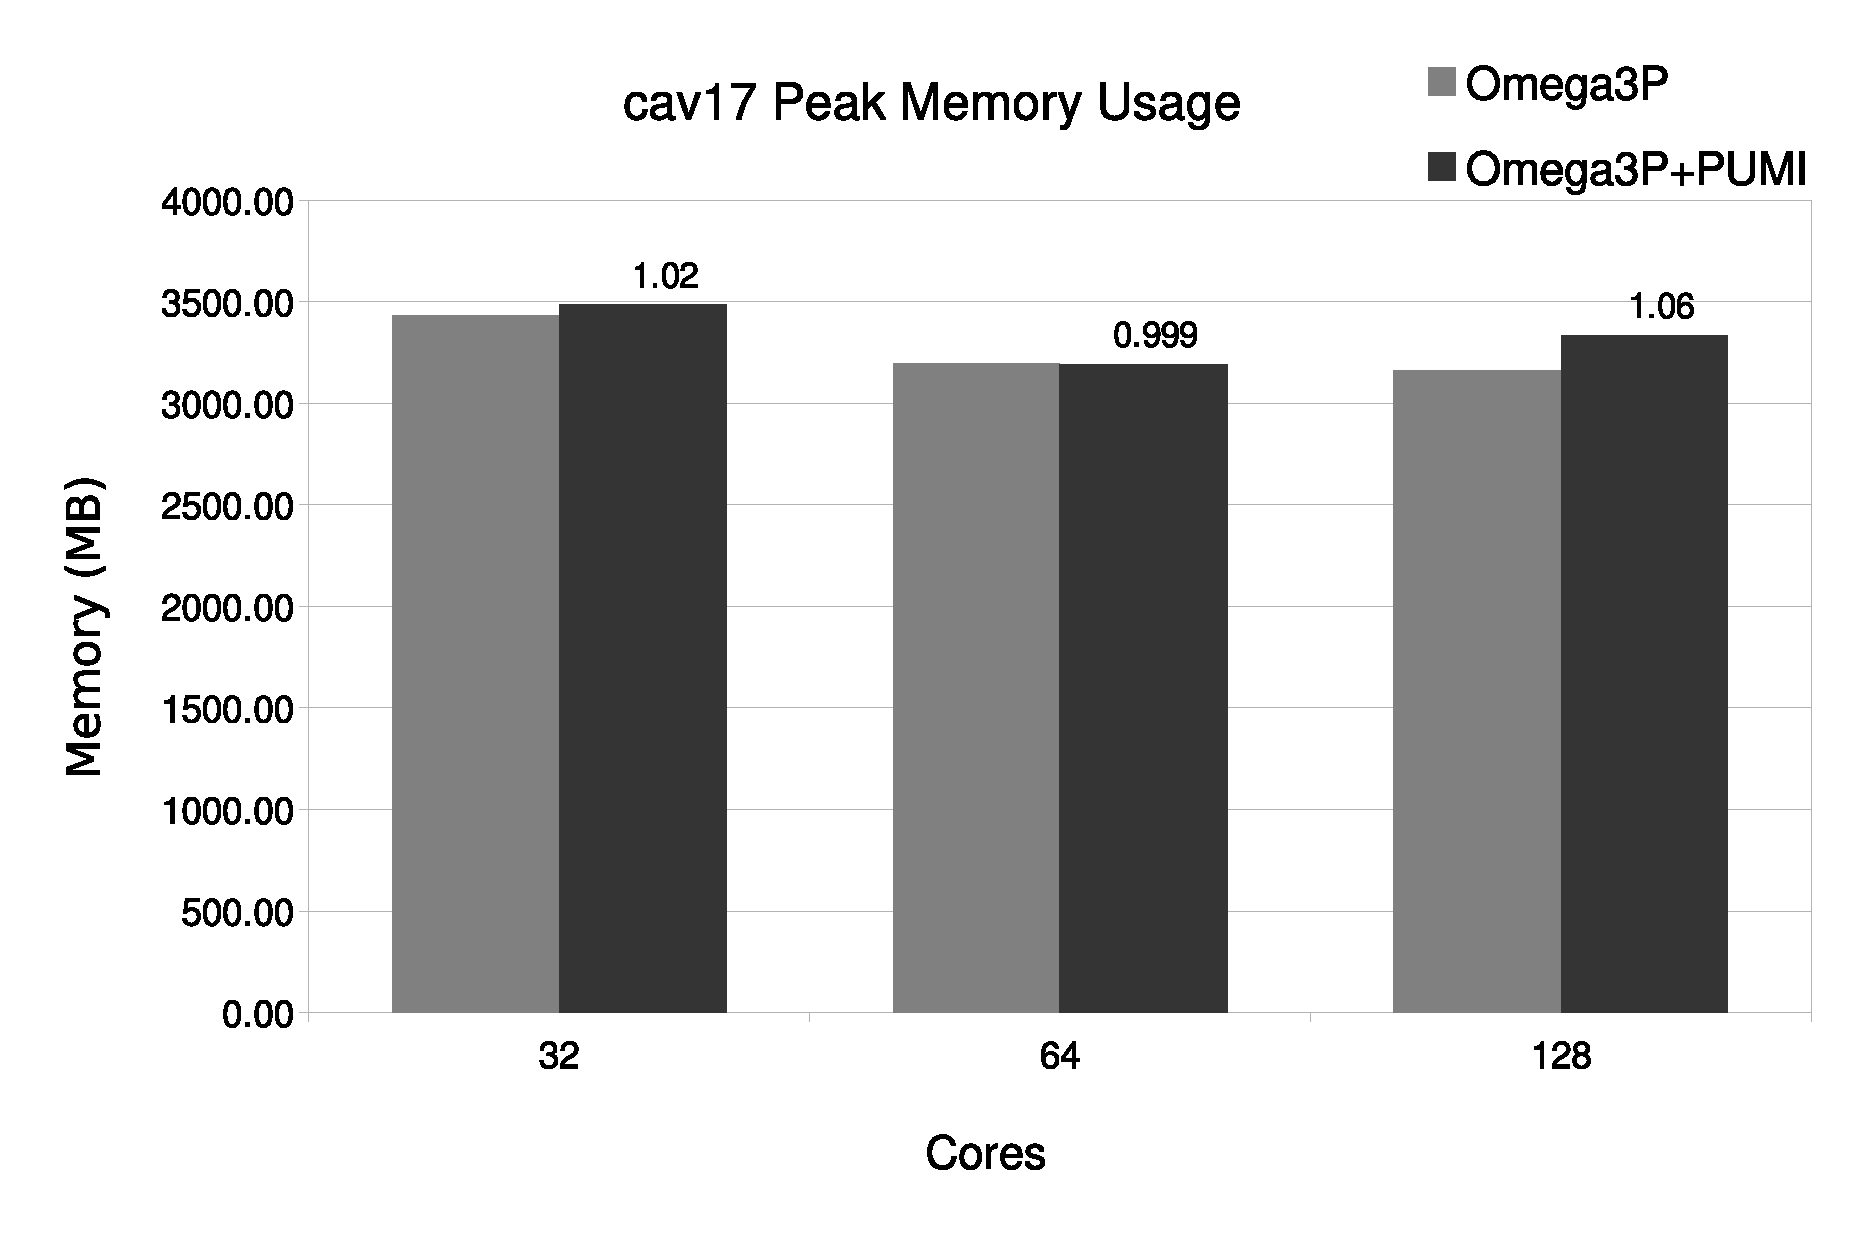
\includegraphics[width=.9\textwidth]{cav17-peak-mem.eps}
  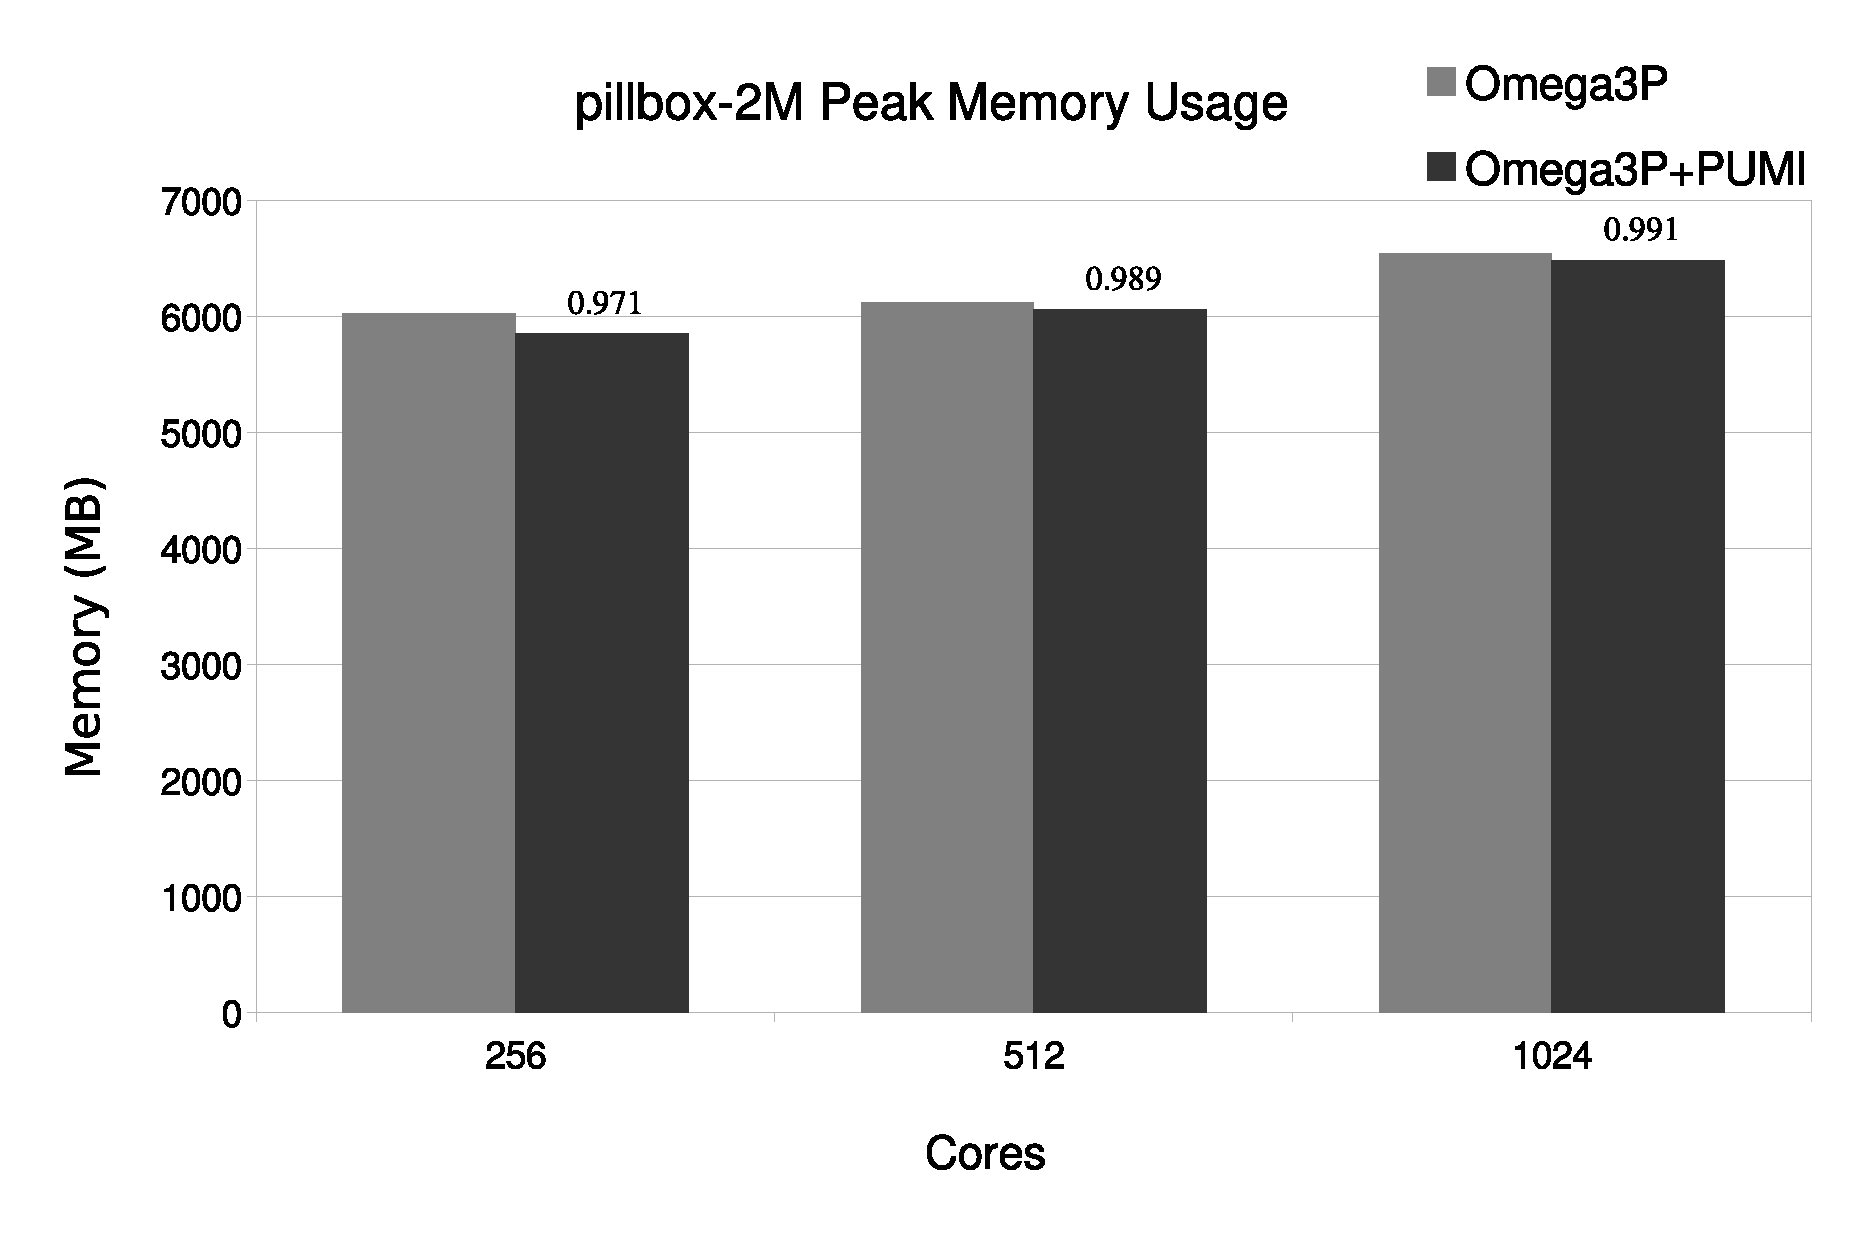
\includegraphics[width=.9\textwidth]{pillbox2M-peak-mem.eps}
  \caption{\label{fig:memusage} Peak memory usage. The labels above the Omega3P+PUMI bars
  list the percent increase versus Omega3P.}
\end{figure}

%\subsection{\label{in_memory_future} Future Steps}
%Our plan for future developments in regard to the in memory integration is as follows:

%\setstretch{0.75}
%\begin{itemize}
%  \item item 1
%  \item item 2
%  \item \dots
%\end{itemize}
\setstretch{1.5}


\section{\label{load_balance}Load Balancing}
In each iteration of the mesh adaptation loop a new partition is generated on the
pumi-mesh before converted over to the slac-mesh. The initial partition is generated
using Zoltan's graph partitioning. Then SCOREC's ParMA, partitioning using mesh adjacencies,
is used to perform load balancing by iterative diffusion. ParMA's multi-entity balancing
traverses an application-specified priority list of entity orders (vertex, edge, face,
region) to balance in descending order.
For each entity order iterative diffusion is executed until balance is reached
or no further improvement is possible.

ParMA's support for multi-entity balancing was extended for Omega3P's needs.
The Omega3P solving step relies on both on-part mesh entities as well as a layer
of ghosted elements along each part boundary.
Omega3P's ghosting uses vertex adjacency such that every element that shares a
vertex with a part boundary will be ghosted to each part that shares that
boundary.
This can be seen in Figure \ref{fig:ghost3} that shows an example of a mesh with
a layer of ghosting.
In order to improve Omega3P's performance and scalability, ParMA targets
minimizing the sum of the ghosted and on-part elements as well as the mesh
entities holding degrees-of-freedom.

\begin{figure}[!ph]
\centering
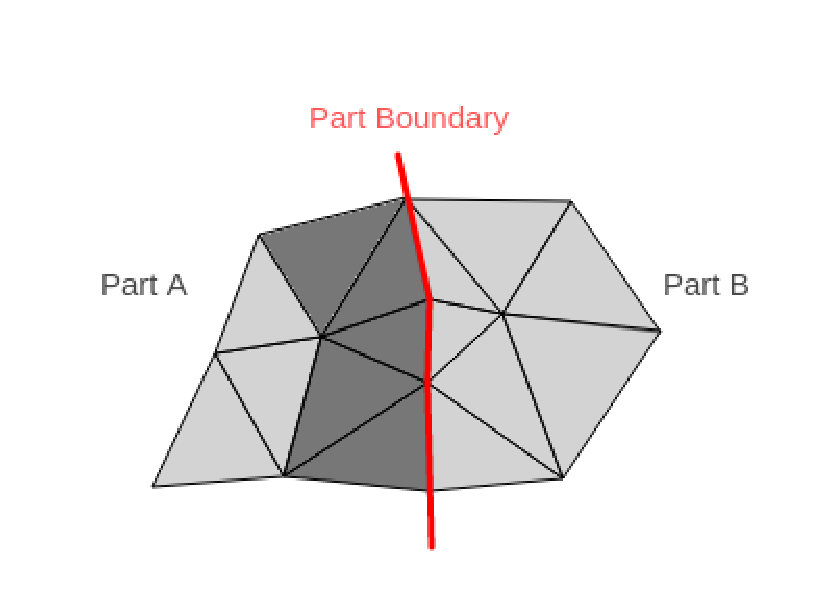
\includegraphics[width=0.6\textwidth]{ghost.eps} 
\caption{\label{fig:ghost3} A layer of ghosted elements from part A to part B. The darker elements represent all the elements on part A that part B will copy to create its remote mesh.}
\end{figure}

ParMA balances the degree-of-freedom holders defined by 
hierarchical Nedelec basis functions~\cite{ingelstrom2006new,ko2010advances} by
reusing existing multi-entity target and boundary-element selection
procedures.
For first order elements this requires balancing edges.
Second order elements requires edges and faces, and above that edges, faces, and
regions need to be balanced. 
Each of these entity balancing procedures accounts for the ghosted weight
contribution by performing an additional neighborhood
exchange~\cite{ibanez2014hybrid} of the exact weight of ghosted layer entities.
Thus ParMA can readily account for balancing the work load, in terms of number
of equations per-part, for p-version finite elements by setting mesh entity
weights based on the different entity p-orders. 

\subsection{\label{load_balance_results} Results}

We ran Omega3P and Omega3P+PUMI on the \texttt{cav17} model with a 318,118
element quadratic mesh on up to 128 cores (32 cores per node) of the NERSC Cori
Phase I system. Two results come from using ParMA's ghost load balancing. The first 
is the improvement of the imbalance of ghost+ owned edges and faces, while the second 
is an increase in average number of ghost+owned entities.
Figure~\ref{fig:cav17imb} shows the imbalance of edges and faces.
At 128 parts ParMA reduces the edge imbalance by 23\%  and the face
imbalance by 14\%.
At 64 parts the edge and face imbalances are reduced by over 12\% each and
at 32 parts ParMA reduces the imbalances by 6\%.
While ParMA significantly reduces the imbalance of ghost+ owned edges and faces
there is a small cost in the number of ghost + owned entities.
The Omega3P+PUMI average number of ghost + owned edges and faces per-part
is less than 1.46\% higher than the Omega3P counts at 32 parts.
At 64 and 128 parts the average entity counts of Omega3P+PUMI is less than 0.3\%
higher than Omega3P counts.

\begin{figure}[!ph]
\centering
  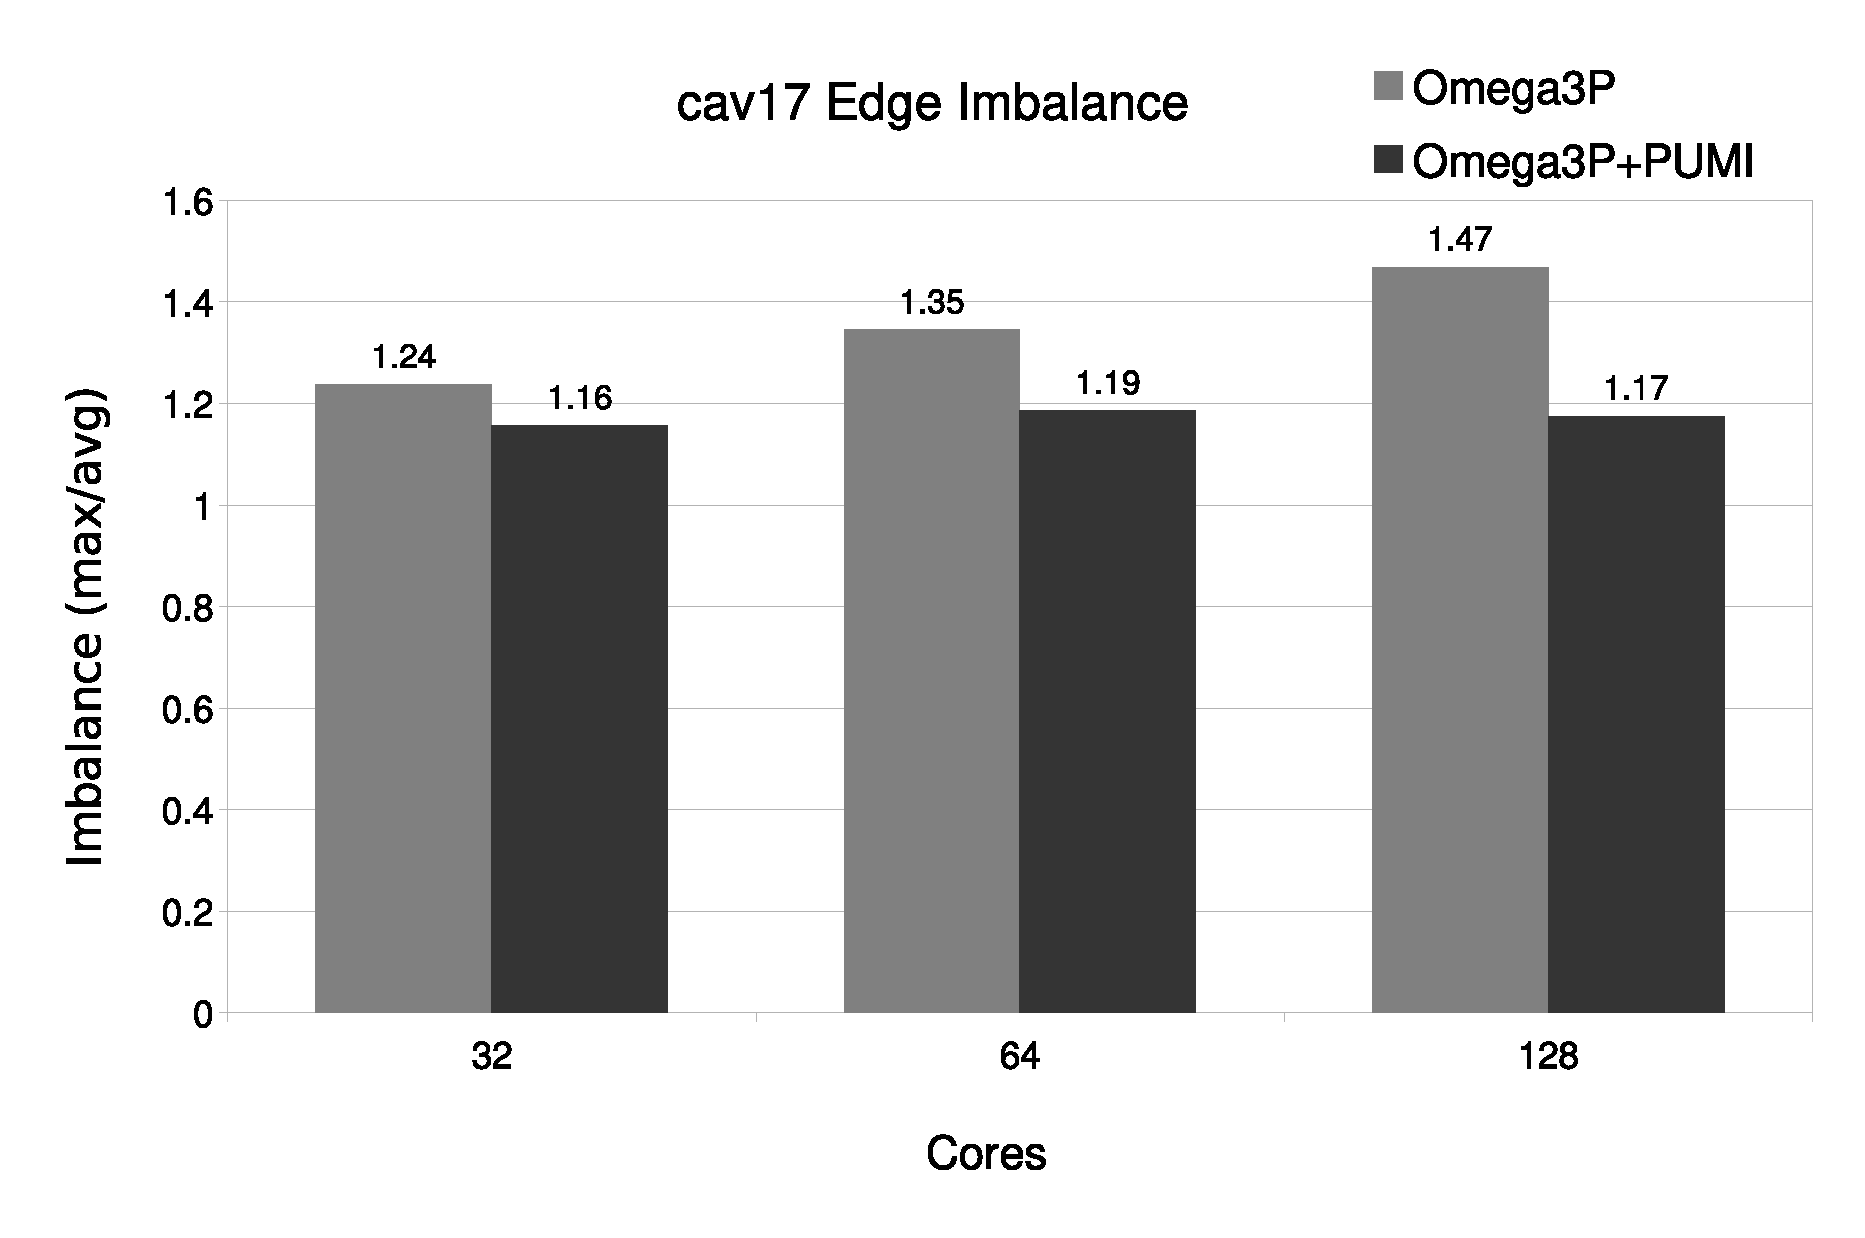
\includegraphics[width=0.75\textwidth]{cav17-edge-imb.eps} \\
  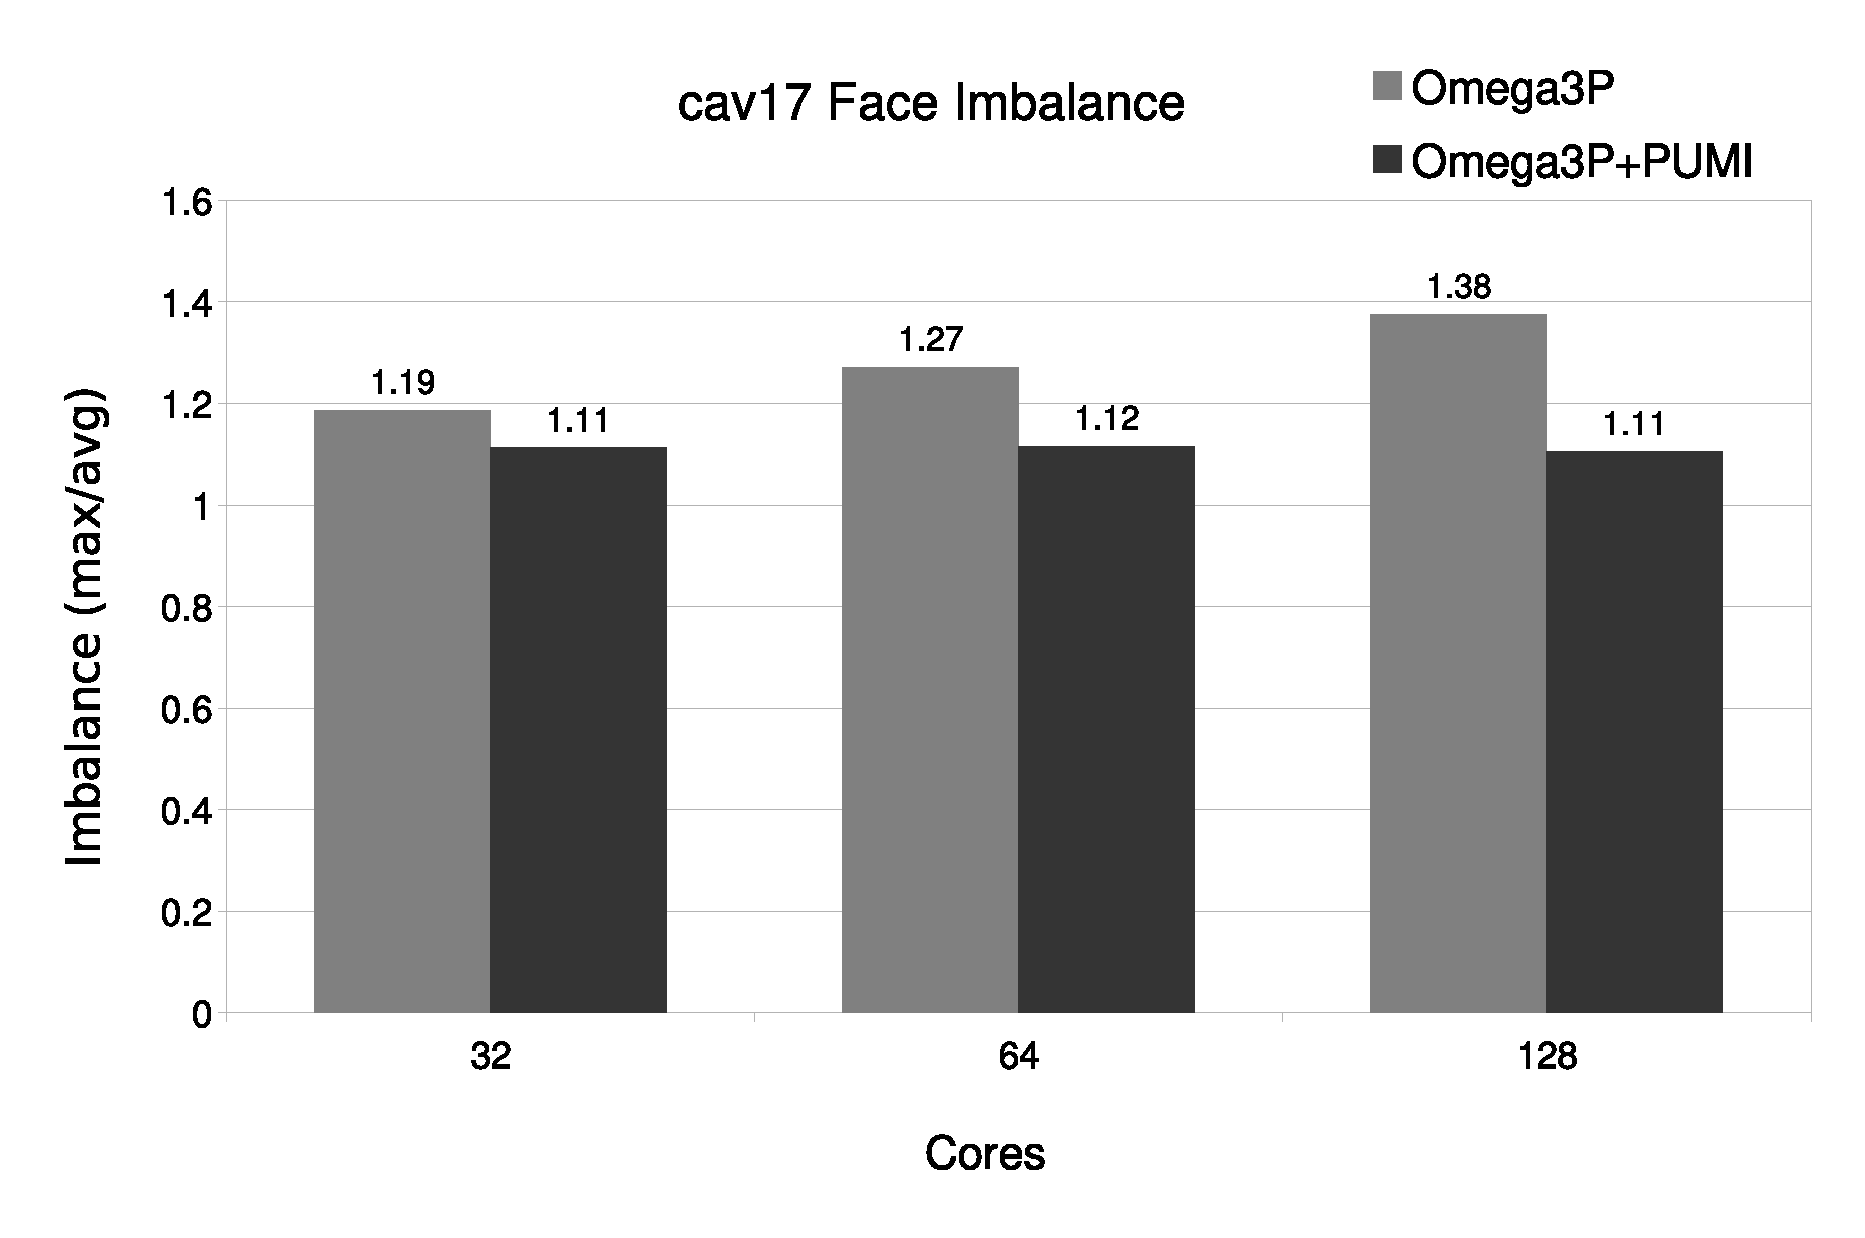
\includegraphics[width=0.75\textwidth]{cav17-face-imb.eps} 
  \caption{\label{fig:cav17imb} Edge and face imbalance in the {\texttt cav17} mesh.}
\end{figure}

Additional tests of ParMA ghost-aware edge balancing were executed on the
\texttt{pillbox} model with a 2 million element quadratic mesh on up to 1024
cores (32 cores per node) of the NERSC Cori Phase I system.
Again we see the two results as in the \texttt{cav17} model, with significant reduciton in 
imbalance with a less significant increase in the number of degree of freedom entities.
At 1024 parts Figure~\ref{fig:pillboximb} depicts the ParMA reduction of the
edge imbalance by 36\% and the face imbalance by 34\%.
At 512 parts the edge and face imbalances are reduced by over 30\% each and
at 256 parts ParMA reduces the imbalances by over 20\%.
The Omega3P+PUMI average number of ghost + owned edges and faces per-part
is less than 1.15\% higher than the Omega3P counts at 256, 512, and 1024 parts.


\begin{figure}[!ph]
\centering
  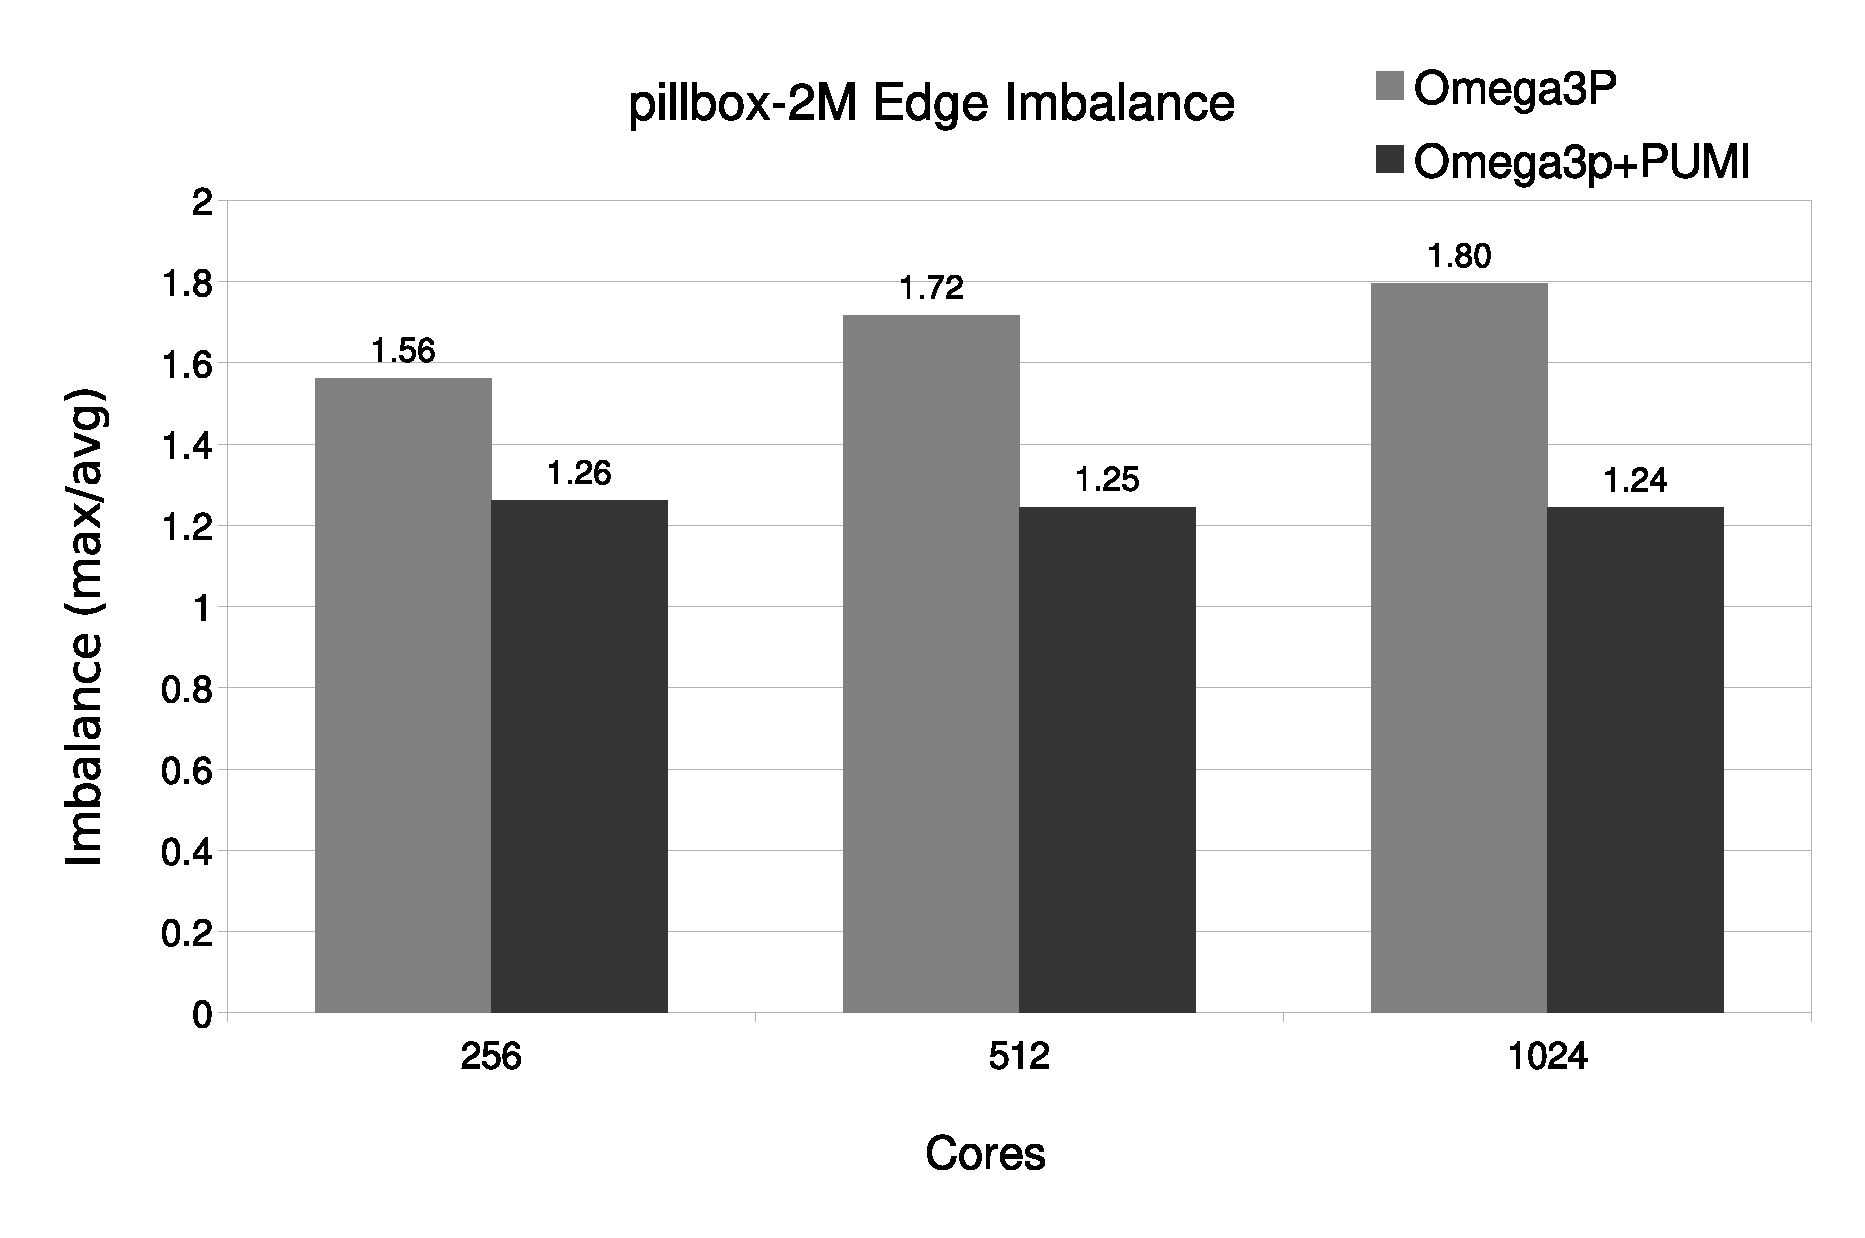
\includegraphics[width=0.75\textwidth]{pillbox2M-edge-imb.eps} \\
  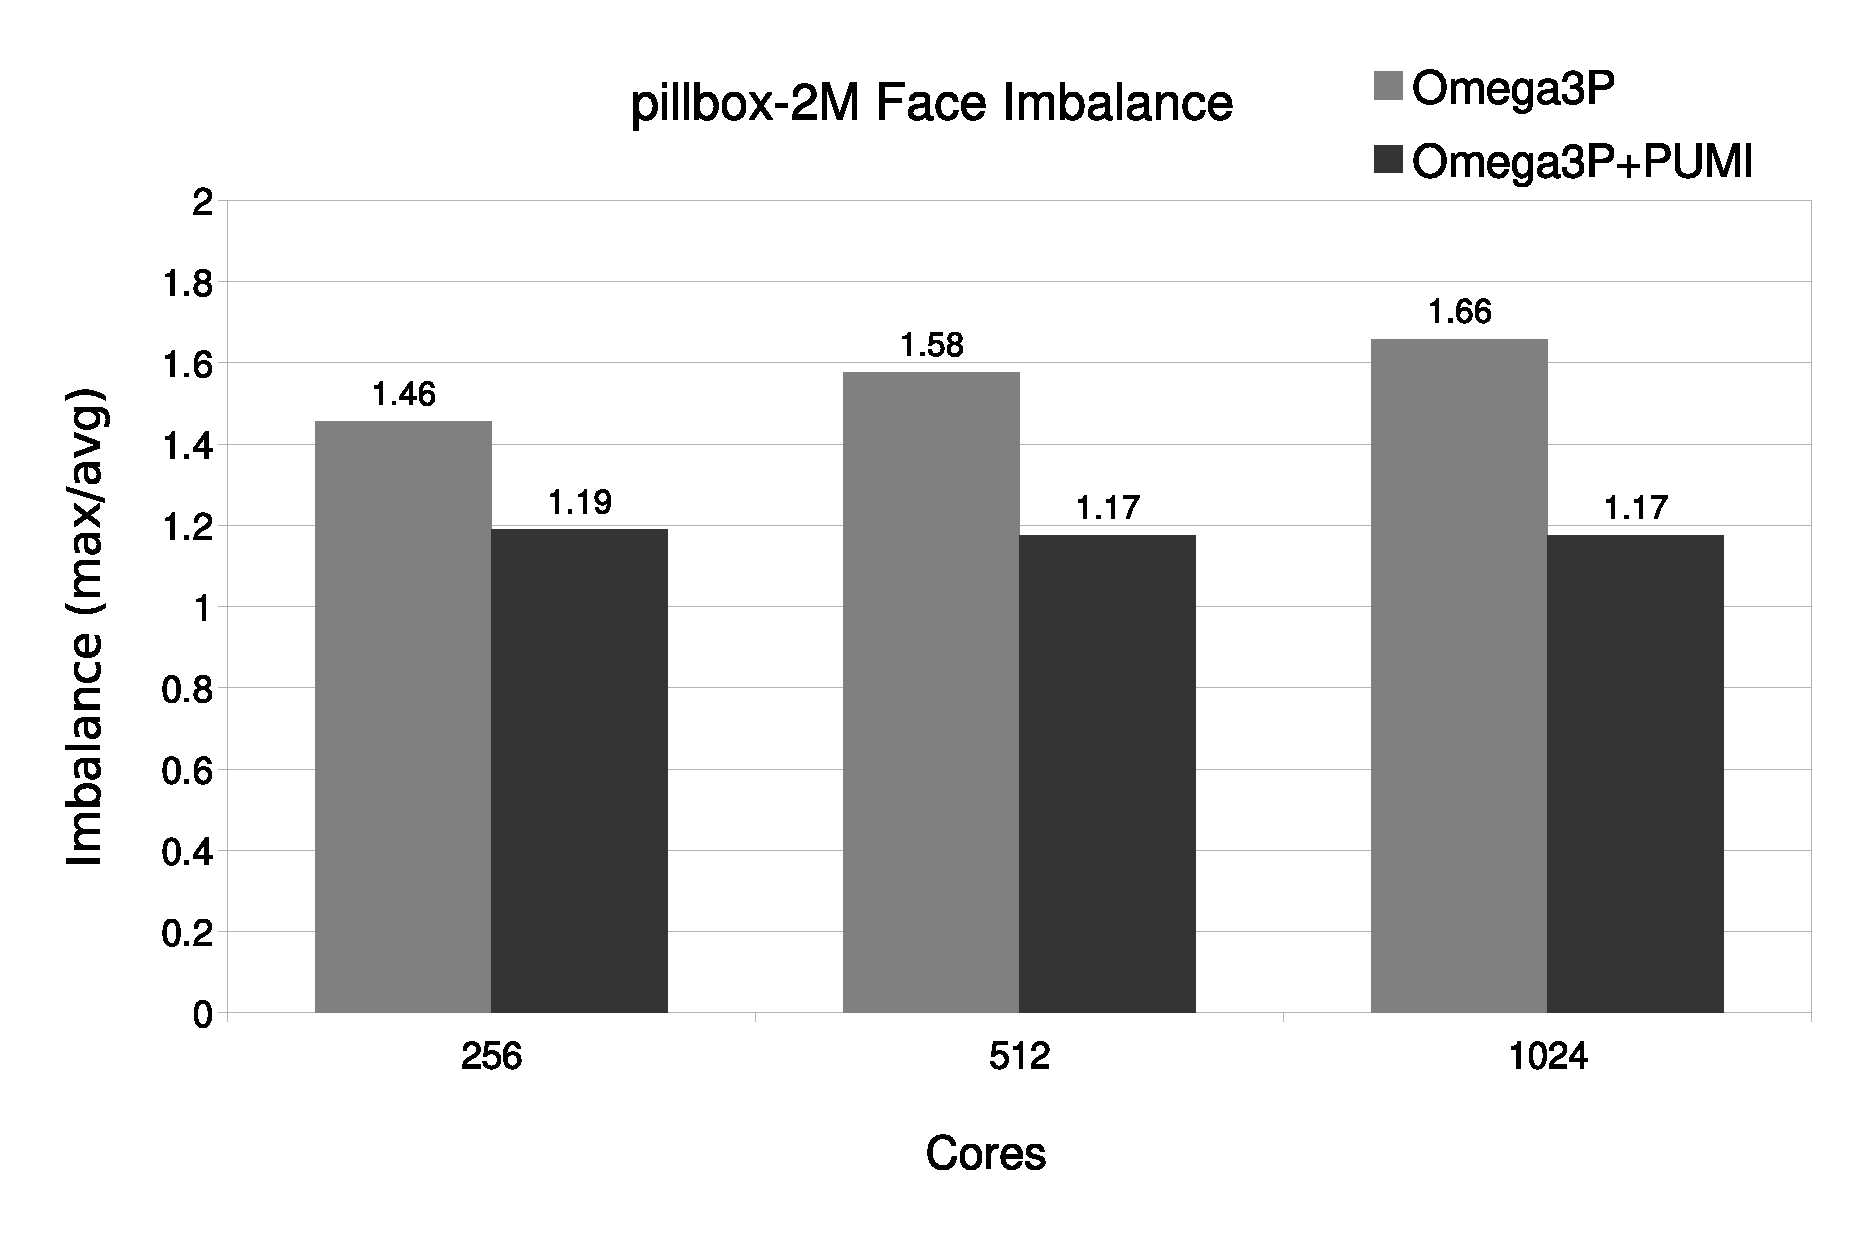
\includegraphics[width=0.75\textwidth]{pillbox2M-face-imb.eps}
  \caption{\label{fig:pillboximb} Edge and face imbalance in the {\texttt
  pillbox-2M}
  mesh.}
\end{figure}

\subsection{\label{load_balance_future} Future Steps}
While we have seen major improvements in the degree of freedom holder imbalance,
we have yet to see an improvement in runtime as a result of the balancing. It has been shown that 
these reductions to the degree-of-freedom holding entities significantly improve the 
performance and scalability of
parallel finite element simulations~\cite{zhou2012unstructured}.
 Thus our plan for future developments in regard to the load balancing  is as follows:

\setstretch{0.75}
\begin{itemize}
  \item Determine how the distribution of degrees of freedom effects the runtime for Omega3P.
  \item Further optimize the ParMA ghost balancer to improve runtime of Omega3P solvers.
\end{itemize}
\setstretch{1.5}


% \clearpage
% \newpage

\section{\label{adaptive_loop}The Adaptive Loop}

For the adaptive loop we use a size-driven mesh adaptation procedure \cite{LiShephard_03}, in which a mesh size metric is defined for the desired size of the elements. Then a series of mesh modifications are applied to achieve the desired edge lengths in the mesh. These operations are:
\begin{itemize}
  \item \textbf{Coarsening}: This stage removes the edges in the mesh that are shorter than the desired edge length. This is achieved by applying collapse operations on short edges.
  \item \textbf{Refinement}: This stage applies edge-based refinement to the mesh in order to achieve the desired edge-lengths. This stage is accompanied by other local mesh modification steps to snap the newly created nodes during the refinement step to the model boundary. They are repeated until the desired sizes are achieved.
  \item \textbf{Shape improvement}: This stage uses operations like edge-swap and vertex repositioning to improve the quality of the mesh. Currently, not implemented for curved mesh adaptation in PUMI.
\end{itemize}
A mesh validity check is performed anytime a local mesh modification is run in places with curved elements to ensure that the resulting elements are not inverted \cite[see][for more details]{LuoShephard_11}. The pseudo-code for the above-described curve adapt procedure is given below.

\begin{algorithm}
\caption{The Curve Adapt}\label{crv_adapt}
\begin{algorithmic}[1]
\Procedure{CurveAdapt}{PumiMesh, SizeField}
\State pre-adapt \textbf{balancing} of the mesh
\State \textbf{fix} invalid elements 
\State \textbf{coarsening}
\State mid-adapt \textbf{balancing} of the mesh
\State \textbf{refinement} and \textbf{snapping to model boundary}
\State \textbf{fix} invalid elements 
\State post-adapt \textbf{balancing} of the mesh
\State \textbf{shape improvement}[currently not implemented for curved mesh adaptation]
\EndProcedure
\end{algorithmic}
\end{algorithm}

With the in-memory integration technique described in section \ref{in_memory}, we always have access to a PUMI-mesh object which enables us to seamlessly \textbf{integrate} the Omega3P's eigen-solvers with different PUMI functionalities, such as load-balancing which was discussed earlier in this report, and adaptations. The following pseudo-code shows the implemented adaptive loop which make use of Omega3P's eigen-solver to compute a size field which is them inputted into the curve adapt procedure described above.

\begin{algorithm}
\caption{The Adaptive Loop}\label{adapt_loop}
\begin{algorithmic}[1]
\State \textbf{while} not converged
\State \quad partition the mesh using ParMA with a focus of owned and ghost elements
\State \quad convert PUMI-mesh to SLAC-mesh
\State \quad run the appropriate Omega3P eigensolver
\State \quad transfer electric field values to the PUMI-mesh
\State \quad check for convergence
\State \quad run Super-convergent Patch Recovery (SPR) error estimator to obtain the size field
\State \quad run CurveAdapt
\end{algorithmic}
\end{algorithm}

Note that our current pipeline works with PUMI-meshes as an input without the need for an input NCDF mesh. This enables us to generate our initial meshes using Simmetrix. Furthermore, the current geometric model inquiries for the purpose of snapping the vertex and mid-edge nodes to the model, requires Simmetrix.

Also worth mentioning, is the fact that our current adaptive loop improves upon the previously available adaptive loop (implemented by Kai) in that it is fully parallel. Recall that the previous implementation required repartitioning a serial mesh after parallel adaptation.

\subsection{Results for the Adaptive Loop}
% \color{blue} Mark: The mesh adaptation procedures are currently doing what looks like a poor job on creating the new mesh topology. This is something we will want to work on when we can get to it. (will likely (1) be a while before we can get to it, (2) take a fair amount of work) \color{black}

% \color{blue} Mark: on subfigures (b) and (d): Why are we plotting such different things? We want the same simulation fields on both. \color{black}

Figures \ref{pill} and \ref{cav} show two working examples for the current curve adaptation loop.
In particular, Fig. \ref{pill} shows the results for the smaller ``PILLBOX''. We start with a uniform and relatively coarse mesh as shown in Fig. \ref{pill_init_mesh}. The desired size field for this initial mesh is obtained based on the magnitude of the electric filed shown in Fig. \ref{pill_init_field}. The resulting size field is plotted in Fig. \ref{pill_init_size}. The final, adapted mesh (for this specific example we needed 3 levels of adaptation) and the final electric field for the first eigen-mode are shown in Figs. \ref{pill_final_mesh} and \ref{pill_final_field}, respectively. Figure \ref{cav} shows the corresponding result for the larger ``CAV17'' model.
\begin{landscape}
\begin{figure}[ph!]
\centering
\subfigure[]{\label{pill_init_field}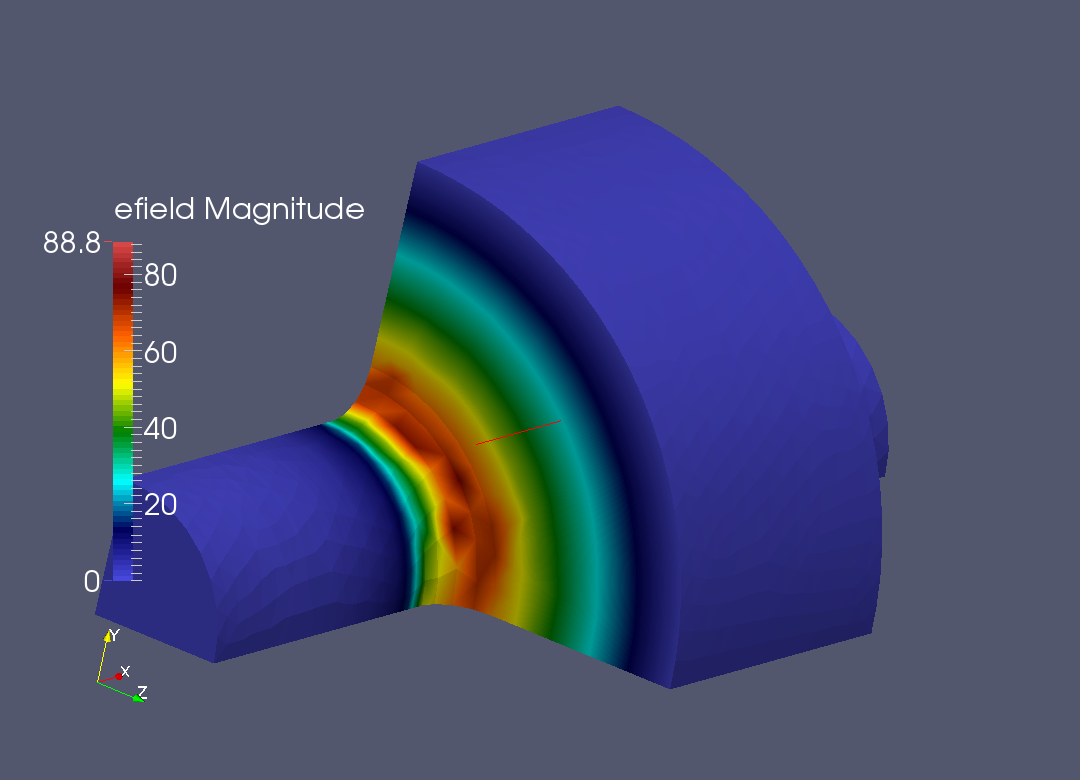
\includegraphics[width=0.55\textwidth]{al_0_ar_0p0125_3721_elems_e_field.png}}
\hspace*{50pt}
\subfigure[]{\label{pill_init_mesh}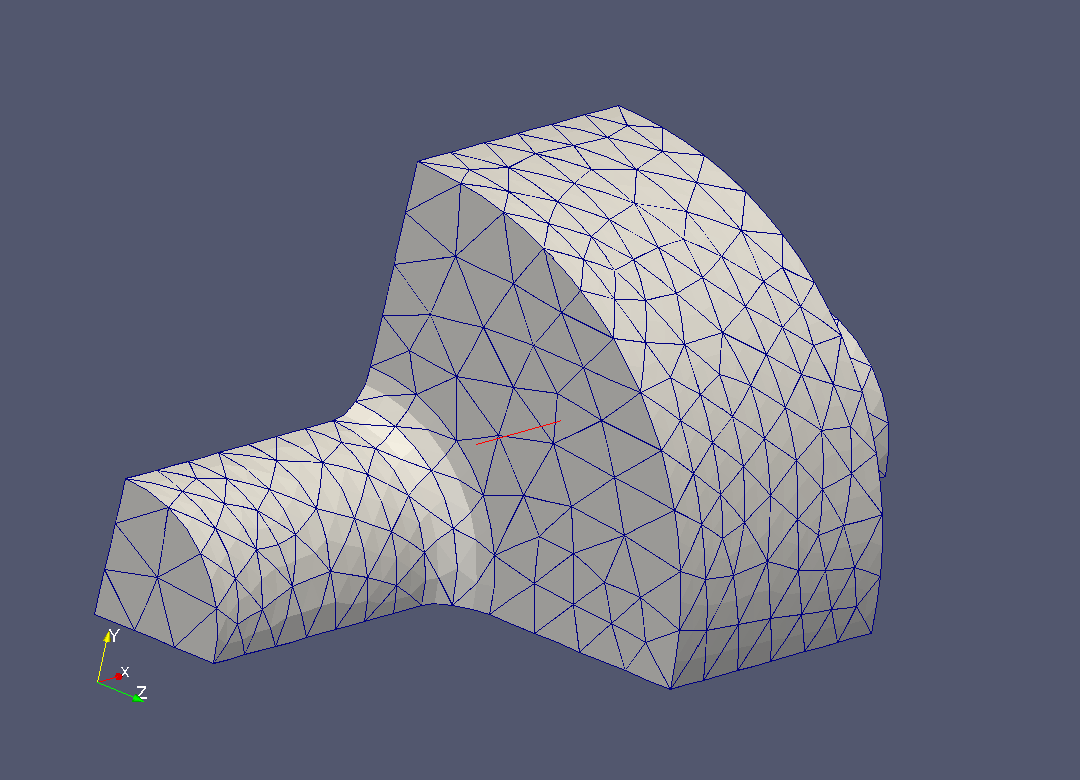
\includegraphics[width=0.55\textwidth]{al_0_ar_0p0125_3721_elems_mesh.png}}
\\
\subfigure[]{\label{pill_final_field}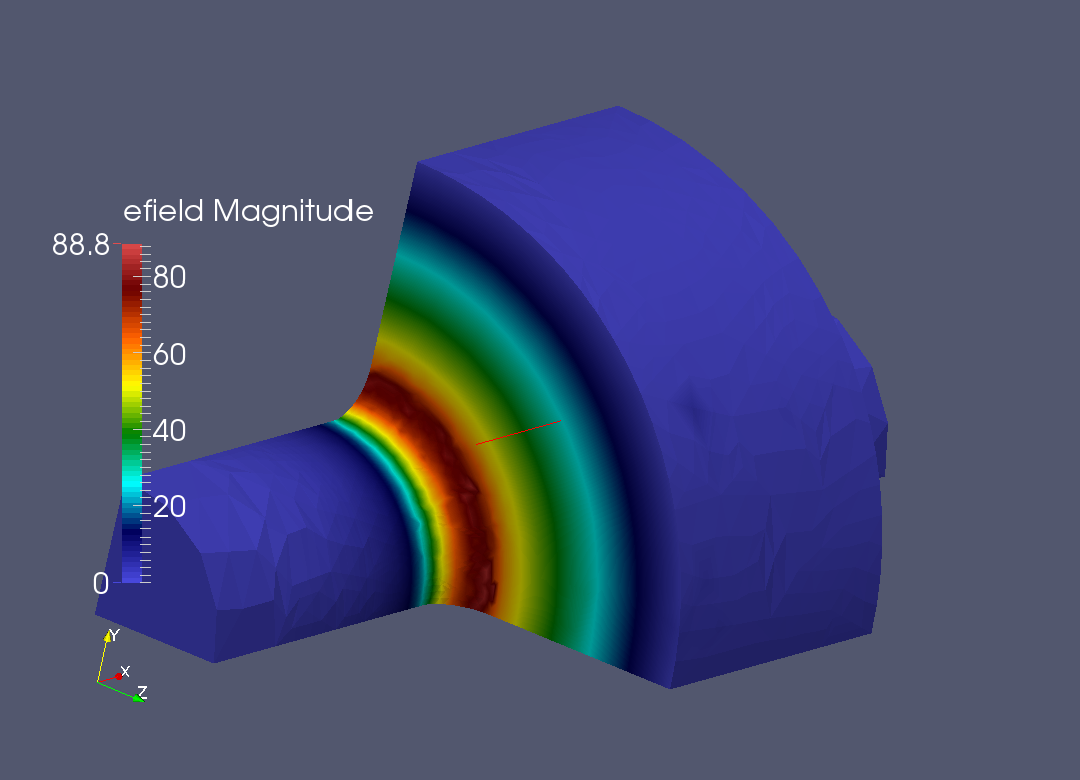
\includegraphics[width=0.55\textwidth]{al_3_ar_0p0125_14221_elems_e_field.png}}
\hspace*{50pt}
\subfigure[]{\label{pill_final_mesh}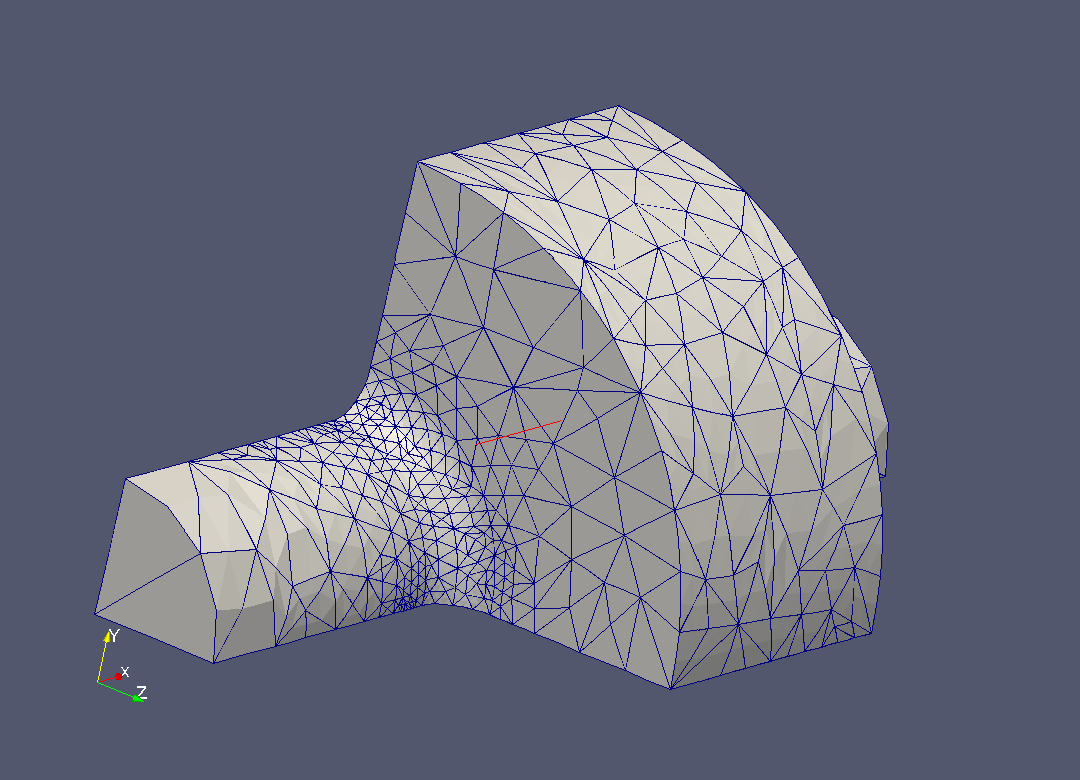
\includegraphics[width=0.55\textwidth]{al_3_ar_0p0125_14221_elems_mesh.png}}
\caption{\label{pill} This Figure shows the results for the PILLBOX model. (a) shows the first eigen-mode electric field on the initial uniform mesh (b) shows the initial uniform mesh [$\sim3.7\text{K}$ elements], (c) shows the first eigen-mode electric field on the final adapted mesh, and (d) shows the final adapted mesh [$\sim14\text{K}$ elements] after 3 adaptation level.}
\end{figure}
\end{landscape}
\begin{landscape}
\begin{figure}[ph!]
\centering
\subfigure[]{\label{cav_init_field}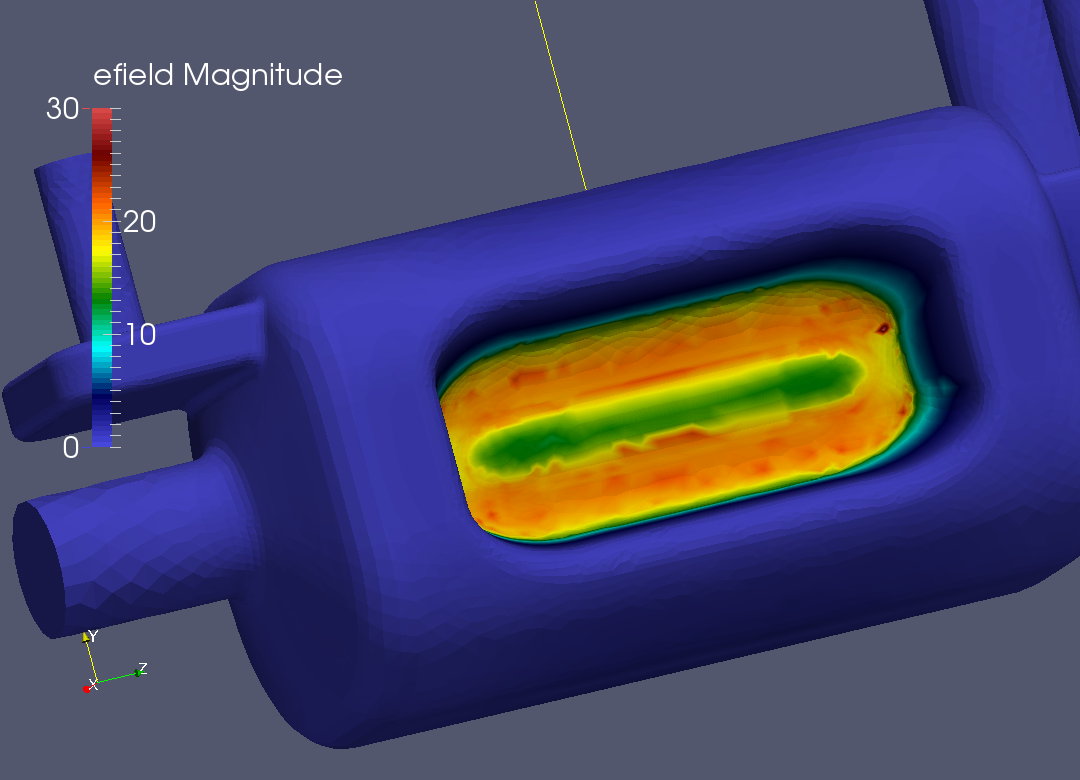
\includegraphics[width=0.55\textwidth]{al_0_ar_0p0125_126044_elems_e_field.png}}
\hspace*{50pt}
\subfigure[]{\label{cav_init_mesh}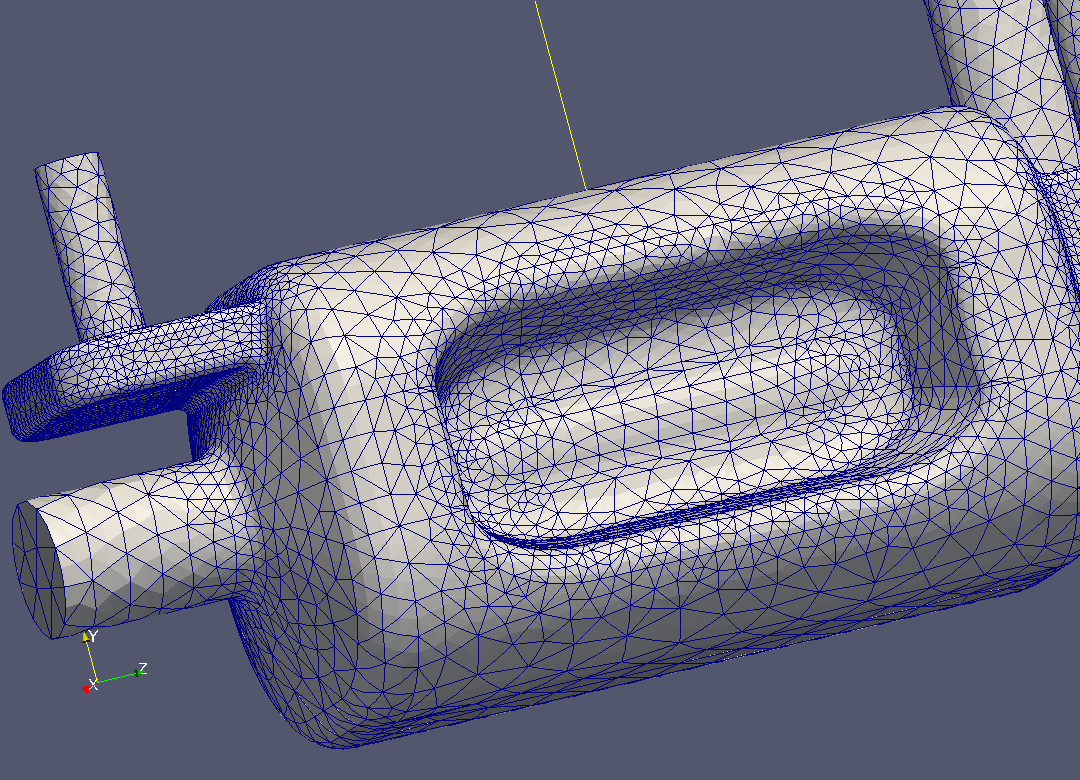
\includegraphics[width=0.55\textwidth]{al_0_ar_0p0125_126044_elems_mesh.png}}
\\
\subfigure[]{\label{cav_final_field}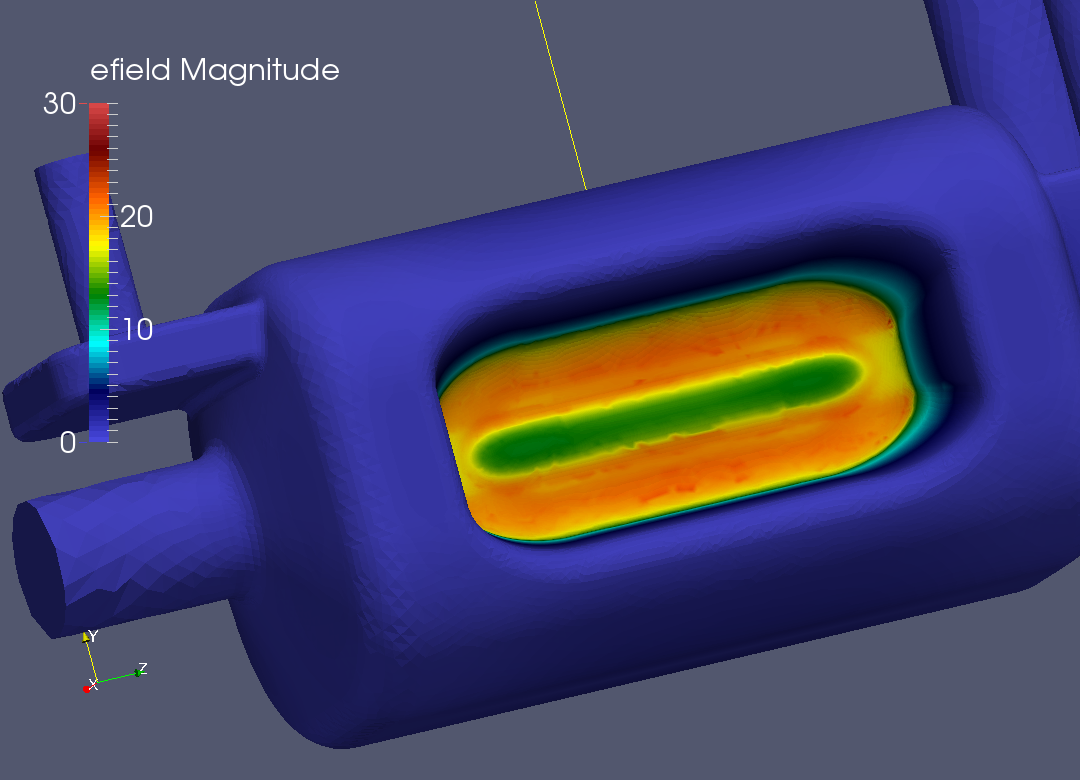
\includegraphics[width=0.55\textwidth]{al_3_ar_0p0125_386896_elems_e_field.png}}
\hspace*{50pt}
\subfigure[]{\label{cav_final_mesh}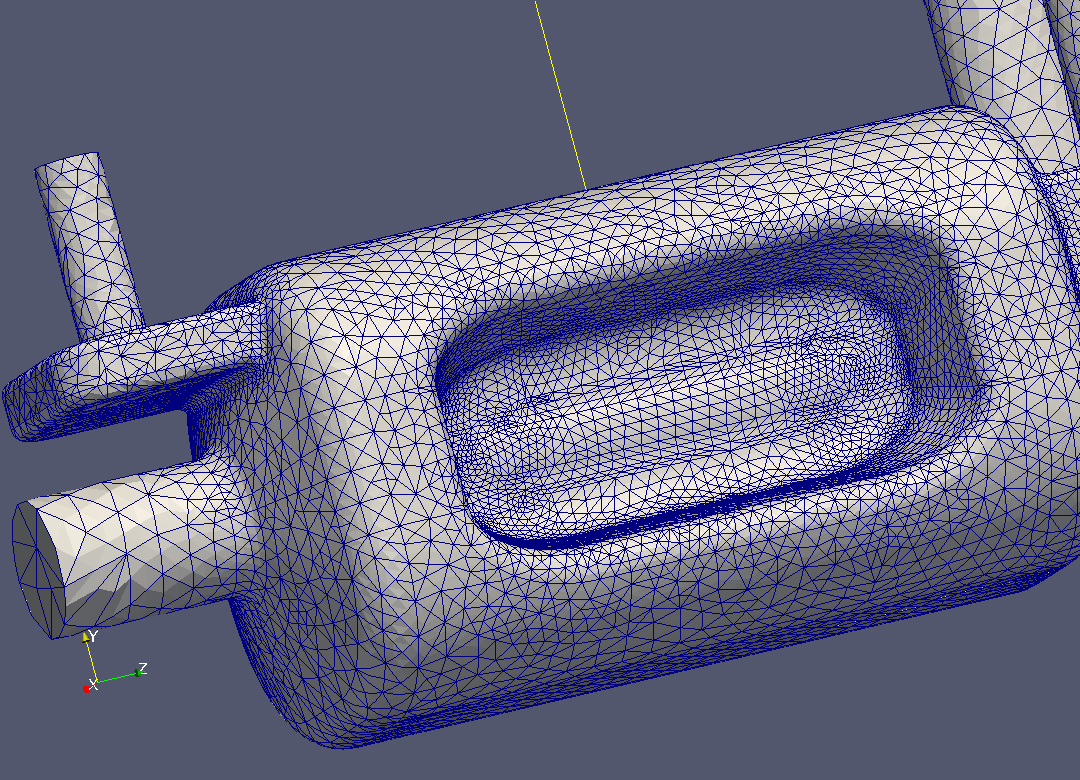
\includegraphics[width=0.55\textwidth]{al_3_ar_0p0125_386896_elems_mesh.png}}
\caption{\label{cav}  This Figure shows the results for the CAV17 model. (a) shows the first eigen-mode electric field on the initial mesh (b) shows the initial  mesh [$\sim126\text{K}$ elements], (c) shows the first eigen-mode electric field on the final adapted mesh, and (d) shows the final adapted mesh [$\sim380\text{K}$ elements] after 3 adaptation level.}
\end{figure}
\end{landscape}
\begin{figure}[ph!]
\centering
\subfigure[]{\label{pill_init_size}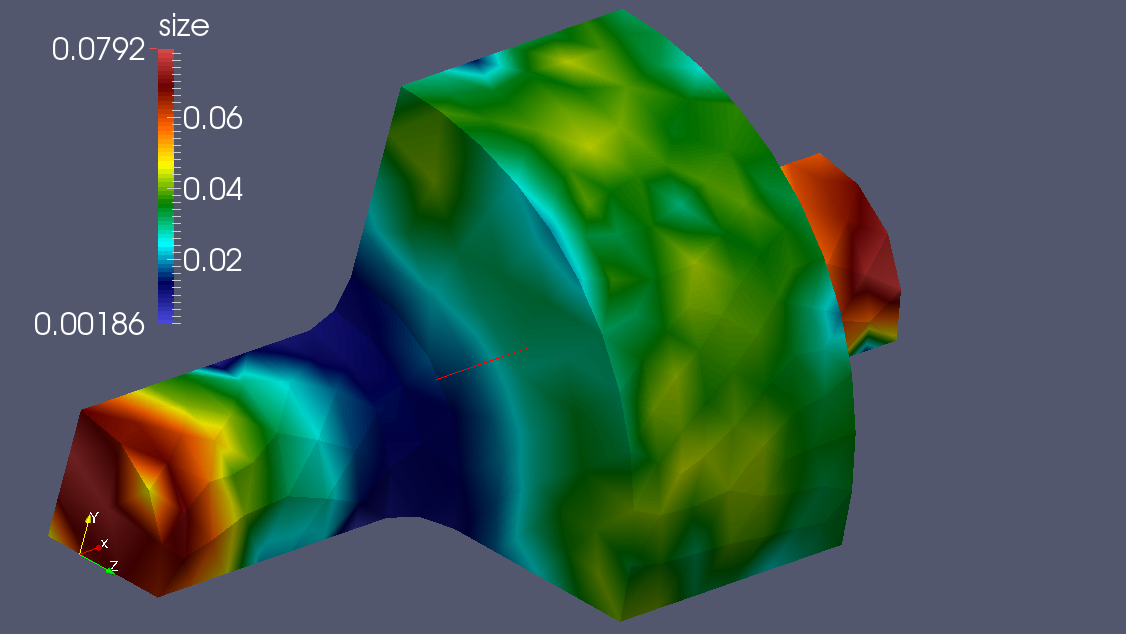
\includegraphics[width=0.75\textwidth]{al_0_ar_0p0125_3721_elems_size_field.png}}
\subfigure[]{\label{cav_init_size}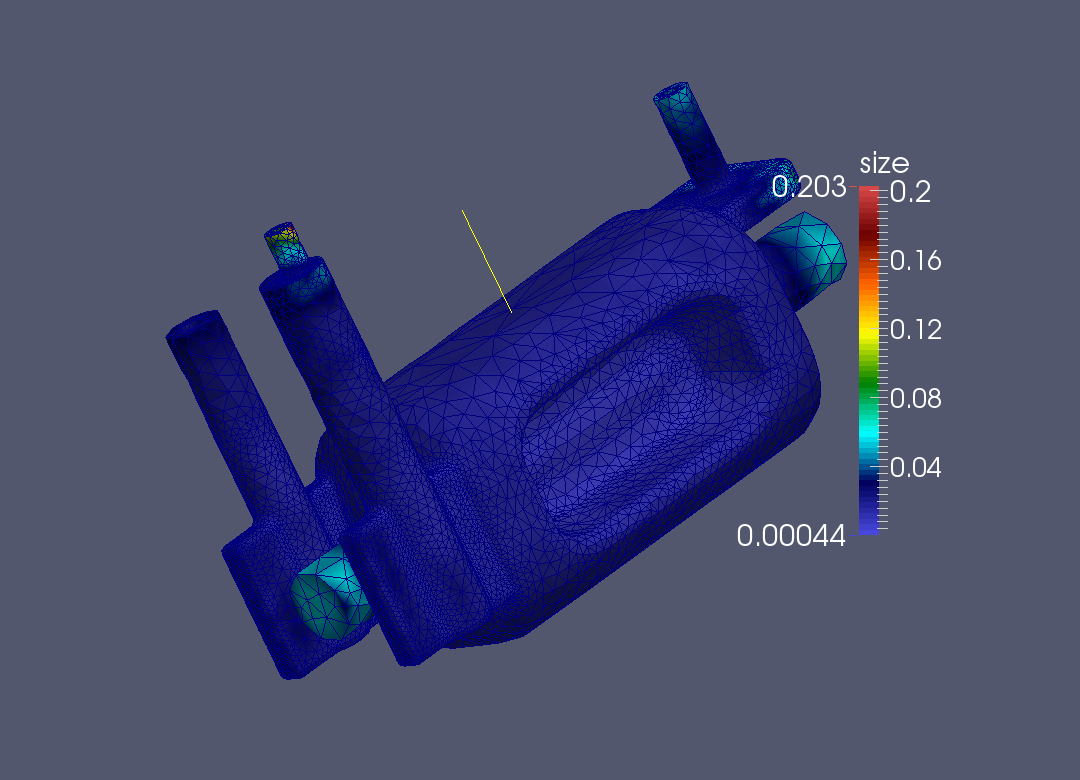
\includegraphics[width=0.75\textwidth]{al_0_ar_0p0125_126044_elems_size_field.png}}
\caption{\label{size_fields} This figure shows the initial size fields for (a) the PILLBOX problem and (b) the CAV17 problem. The size fields are obtained by running the SPR error estimation on the electric electric field in the initial mesh. Note that a new size field is computed at the beginning of each adaptation loop based on the fields values in the pre-adapted mesh, but here we are only showing the initial size fields as a reference for the size distribution in the final adapted mesh with respect to the initial mesh.}
\end{figure}

\subsection{\label{adaptive_loop_future} Future Steps}

Our plan for future developments in regard to the adaptive loop is as follows:
\setstretch{0.75}
\begin{itemize}
  \item Work on the \textbf{shape improvement} step in the adaptive loop for curved meshes in order to be able to produce better quality adapted curved meshes.
\end{itemize}
\setstretch{1.5}



\section{\label{high_order_geom}Moving Towards Higher-Order Geometries}

In order to be able to increase the order of the finite element basis functions to exploit the exponential convergence rate of the p-version finite elements, one needs to also increase the geometric order of the elements near the curved boundaries. Otherwise, the error in the geometric representation of such curved elements prevents the exponential growth rate in the p-version finite element \cite{LuoShephard_04, DeyShephard_97, LuoShephard_02}.

The finite element discretization of the problem involves volume integrals of the form \cite{LeeLi_09}
\begin{equation}
  E^{ij} =  \int _{\Omega _e} \pr{\bs{D} \textbf{N}^i} \cdot \pr{\bs{D} \textbf{N}^j} d\Omega _e	
  \label{integrals}
\end{equation}
where $\Omega _e$ denotes the volume occupied by element $e$ and the operator $\bs{D}$ is either of the following two operators 
\begin{equation}
  \bs{D} \in \cbr{\bs{I}, \bs{\nabla} \times }.
\end{equation}
The element integrals in \mref{\ref{integrals}}, can then be re-written with respect to the parametric coordinates in the reference element. For example, the stiffness matrix for each element can be written as follows
\begin{equation}
\begin{aligned}
  \mu  K^{ij}	&= \int _{\Omega _e} \pr{\bs{\nabla} _x \times \textbf{N}^i} \cdot \pr{\bs{\nabla} _x \times \textbf{N}^j} d\Omega _e \\
  &= \int _{\Omega _e} \epsilon _{kmn} \epsilon_{kpq} \frac{\partial N^i_m}{\partial x_n} \frac{\partial N^j_p}{\partial x_q}   d\Omega _e \\
  &= \int _{\Omega _ {{\xi}}} \epsilon _{kmn} \epsilon_{kpq} \frac{\partial N^i_m}{\partial \xi_s} \frac{\partial \xi_s}{\partial x_n}  \frac{\partial N^j_p}{\partial \xi_t}  \frac{\partial \xi_t}{\partial x_q} \abs{\frac{\partial \mathbf{x}}{\partial \bs{\xi}}  } d\Omega _ {{\xi}} \\
  &= \int _{\Omega _{{\xi}}} \epsilon _{kmn} \epsilon_{kpq} \frac{\partial N^i_m}{\partial \xi_s} J^{-1}_{sn}  \frac{\partial N^j_p}{\partial \xi_t}  J^{-1}_{tq} \abs{\bs{J}} d\Omega _ {{\xi}}.
\end{aligned}
\end{equation}
Here $\epsilon_{kmn}$ is the third-order permutation tensor, and $\mathbf{N}^i$ are the shape functions. Assuming that the Omega3P's code for the computation of the stiffness matrix (or any other matrix pertaining the fem discretization) does not make any specific assumption on the choice of the shape functions, we can safely use other valid shape functions, and  achieve a valid fem discretization. Note that the geometric information of each element is encapsulated in the Jacobians appearing in the above integral, and therefore incorporating higher order geometries into the finite element formulations requires the computation of the Jacobian for higher order elements.

Before moving on to the implementation details, it is worthwhile to mention that for certain type of boundary condition one may need to perform surface integrals over the element faces that fall on the boundary, \cite[cf. section II.E. in][, for example]{LeeLi_09}. Such integrals can also be written in terms of the corresponding integrals in the reference element by using the Nanson's relations
\begin{equation}
  \mathbf{n} dS _x = \abs{\bs{J}} \pr{\bs{J}^{-T}\mathbf{n}'} dS _{{\xi}}
  \label{Nanson}
\end{equation}
where $dS_x$ and $dS _{\xi}$ denote the surface areas in the physical and reference elements, respectively, and $\mathbf{n}$ and $\mathbf{n}'$ denote the corresponding surface normals. As an example, take the following integral which appear is the formulation of the problems with absorbing boundary conditions \cite{LeeLi_09}
\begin{equation}
  \begin{aligned}
    W^{ij} &= \int _{S_x} \pr{\mathbf{n} \times \mathbf{N}^i} \cdot \pr{\mathbf{n} \times \mathbf{N}^j} dS_x \\
    &= \int _{S_\xi} \frac{\br{\pr{\bs{J}^{-T} \mathbf{n}'} \times \mathbf{N}^i} \cdot \br{\pr{\bs{J}^{-T} \mathbf{n}'} \times \mathbf{N}^j}}{\br{\pr{\bs{J}^{-T}\mathbf{n}'} \cdot \pr{\bs{J}^{-T}\mathbf{n}'}}^{1/2}} \abs{\bs{J}}  dS_\xi.
  \end{aligned}
\end{equation}


\begin{figure}[!ph]
\centering
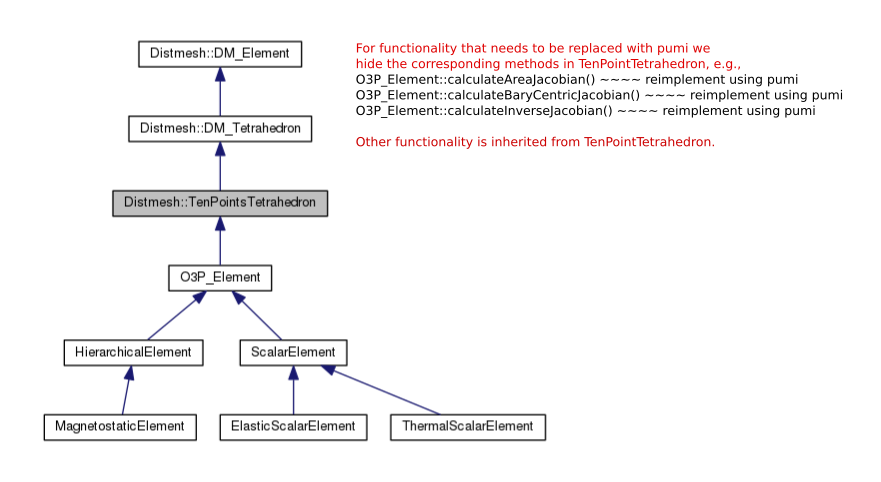
\includegraphics[width=0.95\textwidth]{hide_ten_point_tet.png}
\caption{\label{imp} This Figure shows the implementation details for replacing Omega3P calls for determinant calculation with the corresponding PUMI calls.}
\end{figure}
As a first step towards using higher-order geometric elements, we have been able to replace the Omega3P calls to compute the Jacobian-related quantities (e.g., the determinant) with the corresponding PUMI calls. This is done by storing an additional pointer in each Omega3P-element that points to the corresponding  PUMI-element (see Fig. \ref{imp} for the details of the implementation).
This enables us to easily redirect any call in Omega3P that requires the Jacobians to PUMI and retrieve the corresponding value using the PUMI Jacobian calculations, which supports higher than quadratic geometries. (Currently, we have support for up to 6th order Bezier elements in PUMI.)

\subsection{Results}
By replacing the Jacobian calls in Omega3P with the corresponding PUMI calls we were able to pass the current tests for meshes with quadratic curved  elements, and therefore demonstrate that the above approach works.

\subsection{\label{high_order_geom_future} Future Steps}
Our plan for future developments in regard to the higher-order geometries is as follows:

\setstretch{0.75}
\begin{itemize}
  \item Move to higher order finite element with support for higher order geometries using the approach described above
  \item Once we have full support for higher order geometries we plan to compare the performance improvements of p-version finite element with that of the h-version finite element. 
\end{itemize}
\setstretch{1.5}

\section*{References}
% \bibliographystyle{elsarticle-harv_noURL}
\bibliographystyle{plain}
\bibliography{scorec-refs/partition,scorec-refs/meshdb,scorec-refs/hardware,scorec-refs/io,scorec-refs/frameworks,scorec-refs/cr,scorec-refs/fem,scorec-refs/meshgen,scorec-refs/msgpass,geometry}


\end{document}
